\documentclass[10pt, preprint]{sigplanconf}

% The following \documentclass options may be useful:

% preprint      Remove this option only once the paper is in final form.
% 10pt          To set in 10-point type instead of 9-point.
% 11pt          To set in 11-point type instead of 9-point.
% authoryear    To obtain author/year citation style instead of numeric.

\usepackage{amsmath}
\usepackage{amssymb}
\usepackage{listings}
\usepackage{hyperref}
\usepackage{subcaption}

\special{papersize=8.5in,11in}
\setlength{\pdfpageheight}{\paperheight}
\setlength{\pdfpagewidth}{\paperwidth}

\lstset{captionpos=b, float, language=python}

\usepackage{tikz}
\usetikzlibrary{positioning}
\usetikzlibrary{shadows}
\usetikzlibrary{arrows}
\usetikzlibrary{shapes}
\usetikzlibrary{calc}

\providecommand{\boostsimd}{\textsc{Boost.SIMD}}
\providecommand{\cpp}[1][~]{\textsc{C++}#1}
\providecommand{\ie}[1][~]{\textit{i.e.}#1}
\providecommand{\eg}[1][~]{\textit{e.g.#1}}


\begin{document}


\title{Efficient Compilation of High Level Python Numerical Programs with Pythran}

\authorinfo{Serge Guelton}
           {T{\'e}l{\'e}com Bretagne}
           {serge.guelton@telecom-bretagne.eu}
\authorinfo{Pierrick Brunet}
           {INRIA/MOAIS}
           {pierrick.brunet@inria.fr}
\authorinfo{Mehdi Amini}
           {SILKAN}
           {mehdi.amini@silkan.com}

\maketitle

\begin{abstract}

    For decades, FORTRAN and C(++) have dominated the landscape of High
    Performance Computing languages, leaving interpreted language like Matlab,
    R, Python or more recently Julia for experimentation and prototyping.

    As more scientists use these scripting languages, there is an on-going
    research effort to compile them into efficient native code. However the
    computation kernels often differ from the classical ones as these languages
    favor a high-level coding style, where loops are often replaced by calls
    to the relevant toolbox/module/library/package. As a consequence, traditional
    loop optimization techniques like loop fusion, tiling and related
    vectorization or parallelization techniques are not directly applicable.

    This papers focuses on the case of the Python language and especially the
    Numpy package that provides core array data structure and basic linear
    algebra routines. It first conducts a case study based on Numpy use
    cases from the StackOverflow question and answer website, then studies
    existing compilers for numerical Python. Optimization opportunities,
    including parallelization and vectorization, and their implementation in
    the Pythran compiler are presented and illustrated through several
    benchmarks, showing very interesting speedups over the standard Python
    interpreter. Speedup greater than a factor of 10 are achieved despite the
    fact that the considered benchmarks mostly call Numpy routines that run C code.

\end{abstract}


\keywords
static compilation, parallelization, Python, C++, SIMD


%%
%%
\section{Introduction}
% On aura pas le temps pour le papier je pense mais faire une comparaison avec du
% C pure pour voir ce que les compilo de C arrive a faire.

The Python language~\cite{rossum97} now provides a full toolkit to carry out
scientific experiments~\cite{scipy}, from core scientific routines with the
Numpy package, to scientific packages with the Scipy package, plotting
facilities with the Matplotlib package, enhanced terminal and notebooks with
IPython. As a consequence, there has been a move from historical languages like
Fortran to Python, as showcased by the success of the Scipy conference.

As Python based scientific tools gets widely used, the question of High
performance Computing naturally arises, and it is the focus of many recent
research. Indeed, although there is a great gain in productivity when using
these tools, there is also a performance gap that needs to be filled.

This paper focuses on compilation techniques that are relevant for the
optimization of high-level numerical kernels written in Python using the Numpy
package. Section~\ref{sec:stackoverflow} presents a case study based on user
input gathered on the StackOverflow question and answer site.
Section~\ref{sec:optimize} focuses on a simple yet representative kernel and
showcases the optimization opportunities typically found in Numpy-based
kernels. Existing compilation approach to optimize such kernels are discussed
in Section~\ref{sec:compilers}, then Section~\ref{sec:pythran} emphasises on a
compiler-runtime cooperative approach to solve the performance issues.
Experimentations showcasing important performance gains are detailed in
Section~\ref{sec:xp}.


%%
%%
\section{A Crowd-Sourced Numpy Benchmark}
\label{sec:stackoverflow}

One of the first steps required when designing an optimizing compiler is to
gather enough test cases, or benchmarks, in order to drive the optimization
process toward realistic examples. To achieve this goal, we have gathered a few
example from existing compilers' testsuite, but these may have been modified to
overcome some compiler limitations. A less biased source of benchmarks should
be independant from the compiler community and focused on matching user needs.
To achieve that goal, we collected synthetic scientifc kernels from the
StackOverflow website.

StackOverflow~\footnote{\url{http://stackoverflow.com/}} is a question and
answer site for programmers. Any registered user can submit questions and other
users may answer. A voting system is then used to sort the answers. Said
otherwise, the website provides a database of question and answers on
programming topics, including Python.

A query using the terms \emph{numpy} and \emph{slow} yields many results, many
of which use the pattern ``Q: my code is slow'' followed by an upvoted answer
``A: rewrite it that way'', where the original code performs explicit looping
over an array, and the rewritten code uses the relevant combination of numpy
function.

For instance, question \href{http://stackoverflow.com/questions/7741878}{7741878}
proposes to use an explicit loop to iteratively compute the $L^2$ norm of each
row of a matrix, as illustrated in Listing~\ref{lst:l2norm-loopy}, and one of
the proposed answer is to use the more compact version presented in
Listing~\ref{lst:l2norm}. This answer no longer uses any explicit loops and
roughly achieves a $times 4$ speedup over the loop version.

\begin{lstlisting}[language=python,caption={Per row version of $L^2$ norm with loop in numpy.}, label={lst:l2norm-loopy}]
def slow(x):
    r = np.empty(x.shape[0])
    for i in xrange(x.shape[0]):
        r[i] = np.sum(np.abs(x[i])**2)
    return r
\end{lstlisting}

\begin{lstlisting}[language=python,caption={Per row version of $L^2$ norm without loop in numpy.}, label={lst:l2norm}]
import numpy as np
def l2norm(x):
    return np.sum(np.abs(x)**2, axis=1)
\end{lstlisting}

Our guess is that beginner Numpy users are more likely to make use of raw loops
similar to Listing~\ref{lst:l2norm-loopy}, but as their knowledge of the numpy
API and of the good programming practice grows, they get to write code similar
to Listing~\ref{lst:l2norm}. As a direct consequence, a compiler should
focus on optimizing high-level constructs rather than raw loops. Both to encourage good
practice with respect to Numpy code, and because this is the kind of code Numpy
users ultimately write.

The benchmark is publicly available on
\url{https://github.com/serge-sans-paille/numpy-benchmarks}.


%%
%%
\section{Optimizations Opportunities in a Typical Numpy Kernel}
\label{sec:optimize}

Let us consider the kernel illustrated in Listing~\ref{lst:rosen} and adapted
from the Scipy source code for \texttt{scipy.optimize.rosen}. This kernel makes
use of Numpy's \texttt{sum} function, Python's square notation and Numpy's
array slicing. It is a good example of high-level Python kernel, although
using the function \texttt{scipy.optimize.rosen} would naturally make sense.

\begin{lstlisting}[language=python, caption={High-level implementation of the rosenbrock function in Numpy}, label={lst:rosen}]
def rosen(x):
    t0 = 100 * (x[1:] - x[:-1] ** 2) ** 2
    t1 = (1 - x[:-1]) ** 2
    return numpy.sum(t0 + t1)
\end{lstlisting}

This section goes through all the optimization opportunities in
Listing~\ref{lst:rosen} as a showcase of what an optimizing compiler could do.


\subsection{Temporaries Elimination}
\label{sec:temporaries-elimination}

In Numpy, all point-to-point array operations allocate a new array that holds
the computation result. This behavior is consistent with many Python standard
module, but it is a very inefficient design choice, as it keeps on polluting
the cache with potentially large fresh storage. In the rosen expression from
Listing~\ref{lst:rosen}, 7 temporary arrays are allocated (slicing does not
create a temporary array but a view) to hold intermediate steps. Had the
computation been lazy, no temporary would have been needed.

\subsection{Operator Fusion}
\label{sec:operator-fusion}

As Numpy is a native library mostly written in C, each operator computation is
performed by a function implemented as a loop performing a single operation,
and the operator chaining is done at the interpreter level. This a typical
problem in library design: if only a small set of functions is provided, it
prevents the optimization of multiple operators into a signle specialized
operator, and provided many operator combinations as part of the library yields
better performance to the price of API bloat. In that case, a loop is used for
each temporary computation, plus an extra loop for the \texttt{numpy.sum}
reduction, where a single loop would have been needed.

\subsection{Loop Vectorization and Parallelization}

Even if compiled with vectorization flags on, there would be very little
benefit to generate SIMD instructions for the respective array operations used
by each operator, as the memory load store would have dominated, especially as
Numpy typically operates on double precision floats. In a similar manner,
parallelization of each operator would yield a terrible speedup because a
synchronization fence would need to be issued between each temporary
computation and the loop computation intensity would be very low compared to
the memory pressure implied by two array reads and one array write for a single
binary operator.

On the opposite, if all computation were merged into a single loop, the whole
loop would be trivially vectorizable and parallelizable.
%% I don't get the logic in the previous sentence...
No dependency check is needed as parallelization and vectorization are deduced
from the semantic of the array operations.
%% you still need a dependency test in the absolute, don't you?
%% I'm not sure about what you mean by "deduced"
%% I guess the only reason that allows to get rid of any dependency test is that
%% memory is never updated but new arrays are created?
%% The question is to which point is it still true after "fusion"

%%
%%
\section{Existing Compilation Approach}
\label{sec:compilers}

The success of Python and the development of its large ecosystem triggered
several attempts to improve its execution speed. The most significant basic
block for high performance numerical simulations is certainly Numpy, a
numerical library to manipulate dense arrays. Numerous routines are exposed in
Python and implemented in C, offering close-to-native performance in some cases.
% FIXME: Numpy is part of this section but somehow covered earlier???
%
However, this library-like approach has inherent limitations that were exposed
in the previous section. To address these limitations, several compiler-based
approaches were proposed.

\subsection{Numpy}
\cite{oliphant2007,numpyarray2011}

% Not sure what to add here because of the previous section.

\subsection{Cython}
\cite{cython2010}

%
Cython~\cite{cython2010} is an hybrid Python/C dialect. It extends the Python
syntax with typing information, calls to native functions from third party
libraries, and a limited set of parallelism constructs, such as the possibility
to define parallel loops, but no task parallelism. When possible, it unboxes
Python variables to improve performance. Without type annotations, the
performance improvement is not terrific, but given enough type annotation,
Cython can generates code that runs as fast as its C equivalent, while
maintaining a syntax close to Python.


\subsection{Numba and Parakeet}


The numba~\footnote{\emph{cf}.\ \texttt{https://github.com/numba/numba}}~\cite{numba}
compiler uses additional type information to generate sequential LLVM bytecode.
Parakeet~\cite{parakeet2012} follows an approach similar to numba, that is
Python to LLVM bytecode translation, but limits its scope to the numpy package,
only supporting a small subset of the Python language. Additionally, it supports
implicit parallelism using an implicit mapping between numpy functions and a set
of parallel primitives including \texttt{map}s \texttt{scan}s and
\texttt{reduce}s. These two approaches use Just-In-Time(JIT) compilation and do
not suffer from backward-incompatibility issues. When meeting an unsupported
construct, numba falls back to Python C-API calls, while parakeet raises an
exception.



\subsection{Copperhead}
\cite{copperhead2011}

Copperhead~\cite{copperhead2011} is a functional, data parallel language
embedded in Python. It uses $n$-uplets, NumPy arrays and lists as its core data
structure and prohibits usage of many control-flow operators such as loops,
enforcing the use of the \texttt{map}, \texttt{filter} or \texttt{reduce}
intrinsics to exhibit parallelism. But it can be efficiently compiled to either
CUDA or C++ with calls to the Thrust\footnote{\emph{cf}.
\texttt{http://thrust.github.com/}} library. Python decorators are used to
identify hot-spots that are JIT-compiled to native code.


\subsection{PyPy}
\cite{pypy2009}

Tools such as PyPy~\cite{pypy2009}, a Python interpreter with a tracing JIT, or
Shed~Skin~\cite{shedskin2006}, a Python to C++ compiler are also viable ways to
enhance Python performance. However Shed~Skin does not provide support for
fine-grained parallelism beyond what the standard library proposes. PyPy is
heading toward STM for parallelism support.

%%
%%
\section{Compilers Cooperation}
\label{sec:pythran}

C/C++ have been at the hearth of high performance computing for many years.
Compiler infrasturctures for these languages also have a long history and
implement many optimizations on the control flow graph, basic blocks or
loops~\cite{Aho2006} that limit usage of assembly code to a few hot spots.
Language extensions like OpenMP~\cite{openmp4} provide a convenient parallel
programming model and libraries like Boost.SIMD~\cite{boostsimd} provide good
abstractions for explicit vectorization. Many highly tuned kernels are
available in the form of thid-party libraies like GotoBlas~\cite{gotoblas2008}.

There is no need to reinvent the wheel when compiling numerical Python kernels.
A more profitable approach is to map Python concept to existing ones, or
translate them into existing them. As a consequence, this section focuses on
the translation of Python constructs to efficient C++ constructs. The choice of
C++ instead of C is motivated by the opportunities offered by meta programming
and the interesting similarities between C++11~\cite{isocxx11} features and
Python constructs.

\subsection{Expression Templates}
\label{sec:expression-templates}

Many C++ linear algebra libraries~\cite{eigen,ublas} use \emph{expression
templates}~\cite{expression_templates, et2012} as a way to efficently describe high
level matrix expressions while avoid the creation of intermediate storage.
Additionnaly, it has the same effect as loop fusion, solving the issues
described in \S~\cite{sec:temporaries-elimination} and
\S~\ref{sec:operator-fusion}.

Thanks to variadic templates introduced in C++11, it is possible to write a
generic C++ meta-class that implements the same API as numpy array and provides
all unary and binary operators, as well as the various form of indexing and
slicing. Listing~\ref{lst:rosen-cxx} illustrates the translation of the Python
code from Listing~\ref{lst:rosen} into C++. Altough this version is more
verbose than the Python one, the translation from one to the other does not
raise any particular issue.

This version does not supress all intermediate computations: typically, the
assignments to \texttt{t0} and \texttt{t1} trigger the computation of the right
hand side expression, thus creating two intermediates array. This usual
limitation is motivated by the inability to prove that \texttt{x} is not
modified before \texttt{t0} is read.

\begin{lstlisting}[language=c++, caption={C++11 translated version of Python version for the rosenbrock kernel.}, label={lst:rosen-cxx}, breaklines=true]
typedef typename x::dtype T;
constexpr size_t N = x::ndim;
ndarray<T, N> t0 = 100L * numpy::square{}(x[slice(1L, None)] - numpy::square{}(x[slice(None,-1L)]));
ndarray<T, N> t1 = numpy::square{}(1L - x[slice(None,-1L)]);
return numpy::sum{}((t0 + t1));
\end{lstlisting}

\subsection{Forward Substitution}
\label{sec:fs}

The limitation of expression templates presented in
\S~\ref{sec:expression-templates} is easy to solve at the Python compiler
level, using forward substitution. Typically, forward substitution is
supported by the computation of a dependency graph that itself relies on
read-write effects and alias analysis.

Alias analysis is impossible for Python programs in general, because of late
binding and possible monkey patching. In the context of a static compiler for
numerical programs, it can be assumed that binding is done statically and no
monkey patching is done.  In that context, it is relatively easy to design an
intra-procedural alias analysis thanks to the absence of pointer arithmetic:
the only language construction that can create aliasing is the assignment, thus
a simple control-flow base alias analysis yields accurate results.

The computation of read-write effects involve the annotation of numpy functions
so that the Python compiler knows that most of them do not modify their
argument, and the computation of argument effects for user functions. This can
be done by considering each function individually and looking for the two kind
of constructs that can modify a function argument: indexing and further
function calls.

To interprocedurally compute the read-write effects, intraprocedrual effects
are first computed. Then we create a directed graph $G$ with as many nodes as
functions. Each node contains a list of integer representing the indices of the
formal argument that are modified intra-procedurally. Then we add an edge
between two nodes, labeeld by an integer tuple $(i, j)$ if $i^\text{th}$ formal
argument of the source is passed as $j^\text{th}$ effective argument of the
sink. The goal is to prune all edges from $G$. To do so, given a node $n$ that
writes $i$, any outcoming edge $(i,j)$ can be safely removed, as we know for
sure that the $i^\text{th}$ parameter is written.  Similarly, an incoming edge
$(j,i)$ can be removed and $j$ is added to the source's list. Iteratively
applying this process removes all edges that can propagate a write, the only
remaining edges propagate a read and can be ultmately removed.

Let us illustrate the algorithm on a simple case. Python code source and the
initial effect graphs are illustrated on Figure~\ref{fig:argument-effects}. The
only node wis write effects is \texttt{bar} that writes \texttt{n} through a
subscript. Outcoming edges (1) and (2) can be removed because they are
outcoming edges of \texttt{bar} starting by \texttt{n}. In coming edge (0) ends
by \texttt{n} that is written by \texttt{bar} so it is possible to prune it
while adding the start \texttt{n} to node \texttt{root}. No edge left, and we
know that both \texttt{root} and \texttt{bar} update their argument, but not
\texttt{foo}.

\begin{figure}

    \begin{subfigure}{.5\textwidth}
        \begin{lstlisting}[language=python]
def foo(s):
  return s * 2

def bar(n, m):
  if m:
    n[0] = bar(n, m / 2)
  return foo(n)

def root(r):
  return bar(r, r[0])
        \end{lstlisting}
        \caption{Input Python program.}
        \label{fig:argument-effects-code}
    \end{subfigure}

    \begin{subfigure}{.5\textwidth}
        \centering
        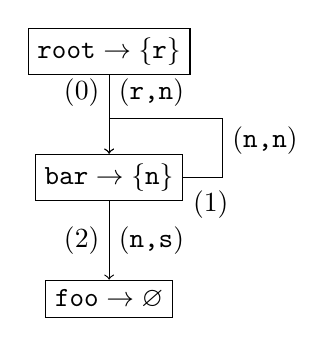
\begin{tikzpicture}[node/.style={rectangle, draw=black}]
            \node[node]  (foo)  {$\texttt{foo} \rightarrow \varnothing$};
            \node[node]  (bar) [above=of foo] {$\texttt{bar} \rightarrow \{\texttt{n}\}$};
            \node[node]  (root) [above=of bar] {$\texttt{root} \rightarrow \{\texttt{r}\}$};

            \draw[->] (bar) -- node[right] {$(\texttt{n,s})$} node[left] {(2)} (foo);
            \draw[->] (bar.east) node[right, yshift=-1em] {(1)} -| ($(bar.east) + (.5,.75)$) node[right, yshift=-.8em] {$(\texttt{n,n})$} -| (bar.north) ;
            \draw[->] (root) -- node[right, yshift=.8em] {$(\texttt{r,n})$} node[left, yshift=.8em] {(0)} (bar);
        \end{tikzpicture}
        \caption{Initial argument effect graph..}
        \label{fig:argument-effects-graph}
    \end{subfigure}

    \caption{Illustration of the argument effect graph (\ref{fig:argument-effects-graph}) of a simple Python program~(\ref{fig:argument-effects-code}).}
    \label{fig:argument-effects}

\end{figure}


\subsection{Range Analysis}

\subsection{Constant Propagation and Loop Unrolling}

There are very few values that are considered as constant in Python, to the
notable exception of strings and tuples. However thare are a lot of constant
propagation opportunities, the most remarkable one being calls to the
\texttt{range} builtin with literal parameters.

A naïve translation of such call to a generic C++ function would generate a
call to a C++ function that would allocate enough memory to hold three integer,
fill the corresponding buffer and return it. A smarter version would generate a
static array holding the relevant values. Figure~\ref{fig:unroll-range}
compares two translation of a Python snippet that iterates over a fixed-size
list. The Clang compiler successfully turns Listing~\ref{lst:stat} into a
single constant. It also statically computes the return value for
Listing~\ref{lst:dyna}, but still generates the intiialization code for the
\texttt{std::vector}. The GCC compiler fails to statically compute the return
value in both cases. This example shows that constant propagation should be
done at a higher level than C++, and so be part of the Python optimizer.

The argument effect analysis described in \S~\ref{sec:fs} can be extended to
global variables to determine if a function as side effects on its argument or
on global variables (including I/O). This information makes it possible to flag
some function as pure, and to statically evaluate pure function calls with
constant arguments. This evaluation is especially easy in Python thanks to the
abitlity of the language to turn an AST expression into bytecode, evaluate it
and retreive its constant value. For instance, this makes it possible to turn a
call to \texttt{range(3)} into \texttt{[0, 1, 2]}, but also to compute the
value of \texttt{fibonnaci(4)} at compile-time.


\begin{figure}

    \begin{subfigure}{.5\textwidth}
    \begin{lstlisting}[language=python]
s = 0
for i in [0,1,2]:
    s += i
return s
\end{lstlisting}
\caption{Python version.}
\end{subfigure}

    \begin{subfigure}{.5\textwidth}
\begin{lstlisting}[language=c++]
long s = 0;
for(auto i: std::vector<long>{{0,1,2}}:
    s += i;
return s;
\end{lstlisting}
\caption{C++ version with dynamic allocation.}
\label{lst:unroll-dyna}
\end{subfigure}

    \begin{subfigure}{.5\textwidth}
\begin{lstlisting}[language=c++]
long s = 0;
for(auto i: std::array<long, 3>{{0,1,2}}:
    s += i;
return s;
\end{lstlisting}
\caption{C++ version with static allocation.}
\label{lst:unroll-stat}
\end{subfigure}

    \caption{Different implementations of an iteration over a fixed size container.}
    \label{fig:unroll-range}

\end{figure}

Once interprocedural constant evaluation is done (eventually followed by
forward substitution), iteration over fixed size lists may appear, giving an
opportunity to fully unroll these loops at the Python level, thus avoiding the
suboptimal C++ translation observed for Listing~\ref{lst:unroll-stat}
and~\ref{lst:unroll-dyna}.

\subsection{Vectorization and Parallelization}

\cite{esterie2012boost, pyhpc2013, wpmvp2014}

%%
%%
\section{Experiments}
\label{sec:xp}

% The first one holds 8 AMD Magny Cours processors for a
% total of 48 cores. Each core has access to 64\,KB of L1 cache,
% 512\,KB of L2 cache. Both L1 and L2 caches are private, while L3 cache
% is shared between the 6 cores of a processor. This configuration
% provides a total of 256\,GB (32\,GB per NUMA node) of main memory. It supports
% up to SSE4. We
% will refer to this configuration as \textbf{AMD48}.
% On AMD48, backend compilers are gcc (Debian 4.7.2-5) and the clang-omp version
% from intel~\footnote{\url{http://clang-omp.github.io/}} to be able to benefits
% from OpenMP improvement. This clang version is based on clang 3.4 release
% (LLVM:233b1e3f034, clang-omp:6f358bcd87).

% The second one holds 8 Intel(R) Xeon(R) CPU E5-2650 0 @ 2.00GHz for a ttal of
% 8 cores (multithreading is not used). Each node can access to  64\,KB of L1 cache,
% 256\,KB of L2 cache. Both L1 and L2 caches are private, while L3 cache
% is shared between the 8 processors. This configuration
% provides a total of 63\,GB of main memory. It supports up to AVX. We will
% refer to this configuration as \textbf{Intel8}.
% On Intel8, backend compilers are gcc 4.9 (20140528) and the clang-omp version
% from intel.

\subsection{The Pythran Compiler}
\cite{pythran2013,isocxx11}


\begin{figure}

    \centering
    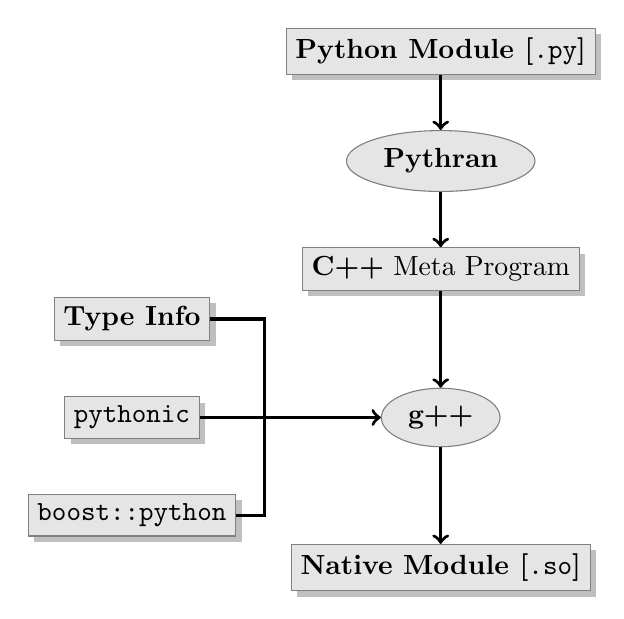
\begin{tikzpicture}[
            file/.style={draw=black!50,fill=black!10,rectangle, drop shadow, align=center,
            node distance=0.7cm},
            tool/.style={draw=black!50,fill=black!10,ellipse, align=center, node
        distance=0.7cm}]
        \node[file] (python) {\textbf{Python Module [\texttt{.py}]}};
        \node[tool] (pythran) [below=of python] {\textbf{Pythran}};
        \node[file] (meta-cxx) [below=of pythran] {\textbf{C++} Meta Program};
        \node[tool] (gxx) [yshift=-1.5em, below=of meta-cxx] {\textbf{g++}};
        \node (empty) [xshift=-1em, left=of gxx] {};
        \node[file] (pythonic) [left=of empty] {\textbf{\texttt{pythonic}}};
        \node[file] (annotation)     [above=of pythonic] {\textbf{Type Info}};
        \node[file] (boost) [below=of pythonic] {\textbf{\texttt{boost::python}}};
        \node[file] (so) [yshift=-1.5em, below=of gxx] {\textbf{Native Module [\texttt{.so}]}};

        \draw[very thick, ->] (python) -- (pythran);
        \draw[very thick] (annotation) -| (empty.center);
        \draw[very thick, ->] (pythran) -- (meta-cxx);
        \draw[very thick, ->] (meta-cxx) -- (gxx);
        \draw[very thick] (boost) -| (empty.center);
        \draw[very thick, ->] (pythonic) -- (gxx);
        \draw[very thick, ->] (gxx) -- (so);
    \end{tikzpicture}

    \caption{Pythran compilation flow.}
    \label{fig:pythran-compiler}

\end{figure}

\subsection{Experimental Setup}

\subsection{Performance of the rosenbrock Function}

\subsection{Results and Analysis}

%%
%%
\section*{Conclusion}

\acks

The Pythran project is an independent Open Source initiative that has been
partially funded by the CARP Project and the SILKAN Company.

Several Students of Télécom Bretagne, namely Adrien Merlini, Alan Raynaud,
Xavier Corbillon, Yuancheng Peng and Eliott Coyacc, have made significant
contributions to the project.

% We recommend abbrvnat bibliography style.

\bibliographystyle{abbrvnat}
\bibliography{biblio}


\end{document}
